%========= Methodology
\section{Python Implementation}

For this report, python was chosen as the coding language. While this choice is largely one of personal preference and accessibility, within the confines of this project collectively our group was supplied with training in python and the advantage of an open source system compared to a licensed system is not one to be ignored. Following along the same path as the methodology, the code was implemented in relation to an image processing, image operation and finally data analysis goal setting.

\subsection{Image Processing}
Briefly consisting of reading the image, splitting the image and binarising the image, this step aims to robustly prepare an input of unknown scale and composition before being passed onto thresholding.

\noindent
To achieve this result, the OpenCV and NumPy libraries were imported. With use of the reading and writing image structures the images were able to be transferred from their original jpg files into 2D arrays containing the greyscale values of their pixels as their representative cells (Fig.\ref{fig:ReadingCode}). From this point onwards, to enhance quality of images passed between functions and to the user, all image files will be saved as a lossless png format.

\begin{figure}[h] %  figure placement: here, top, bottom, or page
    \centering
    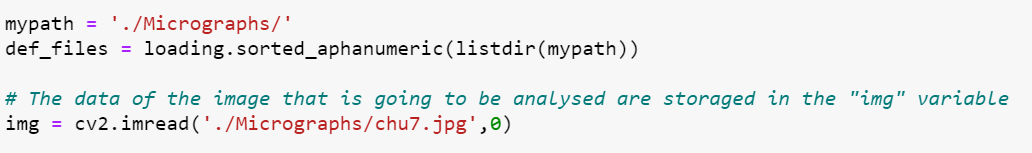
\includegraphics[width=6in]{Figures/Code/Reading an image.png}
    \caption{Screenshot of the code for defining a directoy containing micrographs and reading an image with OpenCV}
    \label{fig:ReadingCode}
\end{figure}


\noindent
Now that the image has been transformed into a form of data manipula